%Present/motivate key ideas/decisions, design options, alternatives, trade-offs.
%Draw architecture block diagram (= picture!).

\seqfilter
We start with the block diagram for one stage in the previous assignments.
This diagram is given in Figure~\ref{fig:design:parallelstage}.

\begin{figure}[h]
	\centering
	\def\svgwidth{0.6\textwidth}
	\input{imgs/parallelstage.pdf_tex}
	\caption{Block diagram for one stage in the previous assignments}
	\label{fig:design:parallelstage}
\end{figure}

In the sequential implemention, we need the previous 32 $b_{out}$ values to compute the current $b_{out}$.

A key challenge is that we cannot just run the entire computation for a value at once, since that would mean a computation step that takes too long, meaning we wouldn't be able to run at 100MHz.
To overcome this, we run one of the 32 steps of the computation each cycle.
Then, in the \th{32} cycle, we write the $b_{out}$ value of the last computation to the \texttt{data\_out} wire.

The coefficients, $h_{in}$ are given as one 512-bit value.
It is too expensive to extract the proper index from this value each computational step, so we read $h_in$ into a buffer \texttt{h\_in\_buf} that contains the 32 values of $h$.
This way, we can access them during the computation with just their index, without having to multiply with the number of bits in one of the values.

We keep a rotating buffer of all current input values ($a$) and $b$ values.
We rotate these arrays by keeping a pointer (\texttt{i}) to the value we are currently working with, and increasing this pointer when we receive new input.
When the pointer wraps, we start overwriting old values that we no longer need for the computation.
We also keep a computational pointer (\texttt{comp\_ptr}), that is initialized at the current input pointer each time we get input.

Each computational step, we first increase the computational pointer, and then perform the basic filter stage computation:

\[
	b[\texttt{comp\_ptr}] = h[i] * a[\texttt{comp\_ptr}] + b[\texttt{comp\_ptr} - 1]
\]

After 32 of these steps, the computational pointer is back at the input pointer, meaning we compute the output for the current given input last.
When this final computation is done, we are ready to put the value of $b$ for the current pointer in the output.

Figure~\ref{fig:design:compstep} shows a block diagram for a computational step (with 11 stages instead of 32).

\begin{figure}[h]
	\centering
	\def\svgwidth{0.6\textwidth}
	\input{imgs/compstep.pdf_tex}
	\caption{Block diagram for one computational step}
	\label{fig:design:compstep}
\end{figure}

As shown, each computational step only uses one multiplier and one adder.
Since the steps run in sequence instead of in parallel, this means our entire design only uses one multiplier and one added.

In the implementation of this design, to speed things up, we have changed a number of things.
Most notably, the buffer for $b$ we use holds only two values, since we are actually only using two at a time.
We have also added an extra delay in the computational step, to make the critical path shorter.

All pointers have been refactored into a single one, \texttt{count}.

Instead of reading the $h$ values into a buffer when we reset, we use the values from the wire directly.
This means we can adhere to the requirement to honor changes in $h$.

\strengthfilter

To design the strength-reduced filter, we first need to apply a strength-reduction to the formula of the filter, as in assignment T4.
We start with the filter:
\begin{align*}
	y(n) &= \sum_{i=0}^{32} h(i)x(n-i)\\
	&= \{\textnormal{Separate odd/even terms}\}\\
	y(n) &= \sum_{j=0}^{16} h(2j)x(n-2j) \\
	&+ \sum_{j=0}^{16} h(2j+1)x(n-2j-1) \\
	&= \{\textnormal{Block processing,} L=2, n=2k\}\\
	y(2k) &= \sum_{j=0}^{16} h(2j)x(2k-2j) \\
	&+ \sum_{j=0}^{16} h(2j+1)x(2k-2j-1) \\
	y(2k+1) &= \sum_{j=0}^{16} h(2j)x(2k+1-2j) \\
	&+ \sum_{j=0}^{16} h(2j+1)x(2k-2j) \\
	&= \{\textnormal{Rewrite}\}\\
	y(2k) &= \sum_{j=0}^{16} h(2j)x(2(k-j)) \\
	&+ \sum_{j=0}^{16} h(2j+1)x(2(k-2j-1)+1) \\
	y(2k+1) &= \sum_{j=0}^{16} h(2j)x(2(k-j)+1) \\
	&+ \sum_{j=0}^{16} h(2j+1)x(2(k-j)) \\
	&= \{\textnormal{Add/substract same terms}\}\\
	y(2k) &= \sum_{j=0}^{16} (h(2j)+h(2j+1)) x(2(k-j)) \\
	&+ \sum_{j=0}^{16} h(2j+1) (x(2(k-j-1)+1) - x(2(k-j))) \\
	y(2k+1) &= \sum_{j=0}^{16} h(2j)(x(2(k-j)+1)-x(2(k-j))) \\
	&+ \sum_{j=0}^{16} (h(2j)+h(2j+1))x(2(k-j)) \\
\end{align*}

$y(2k)$ and $y(2k+1)$ are 16-stage FIR filters.
Since the filters have a term that is the same (the second term of $y(2k)$ is the same as the first term of $y(2k+1)$), we can use these to construct the strength-reduced filter.
Figure~\ref{fig:design:strength}, from the slides, shows how this works.

\begin{figure}[h]
	\centering
	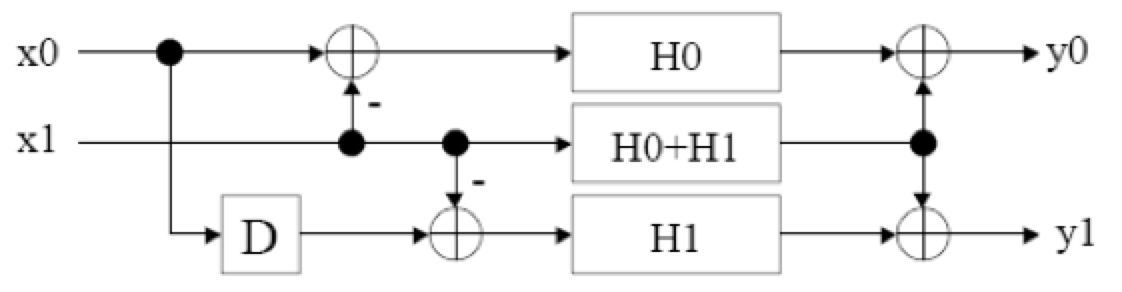
\includegraphics[width=0.6\textwidth]{strength}
	\caption{Block diagram showing how the strength-reduced filter works}
	\label{fig:design:strength}
\end{figure}
